\graphicspath{{content/1_literatureReview/figures/}}
\section{Ultrasonic Sensor Interface}\label{sec:ultrasonicSensorInterface}

The HC-SR04 ultrasonic ranging module will be used. It has 4 pins, namely \textit{$V_{cc}$, GND, Trig (Trigger)} and \textit{Echo}.
It should be powered with 5 ${V_{dc}}$ and requires at least 15 mA to function, meaning it will dissipate 75 mW of power. 
First, \textit{Trig} should be pulled high to indicate that the device should send a burst of ultrasonic sound out.
Then, if the sound wave is received back, the device will output a distance-proportional pulse on the \textit{Echo} pin.

\begin{figure}[!htb]
  \centering
  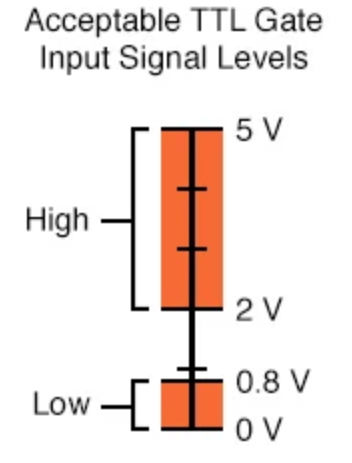
\includegraphics[width=0.15\textwidth]{sonicSensor_TTL}
  \caption{TTL Input/Output Levels \cite{ttlLevels}}
  \label{fig:sonicSensor_TTL}
\end{figure}

The following detailed procedure should be followed to make a distance measurement \cite{datasheetHCSR04}, as also indicated in Figure \ref{fig:sonicSensor_timing}:
\begin{enumerate}
    \item A pulse of at least \SI{10}{\micro\second} should be output onto \textit{Trig}. This pulse must be TTL compliant as indicated
    in Figure \ref{fig:sonicSensor_TTL} i.e. between 2 V and 5 V.
    \item If the sound wave is received back by the sensor, \textit{Echo} will go high (TTL) for ${t_{high}}$ seconds, where ${t_{high}}$ is the time it took the signal to return to the sensor.
          This signal should therefore be conditioned if a circuit which requires 3.3 V is used.
    \item The distance can then be calculated. One of the following methods may be used:
    \begin{enumerate}
        \item The length of time of the \textit{Echo} output signal can be digitally measured and the distance calculated using \inlineequation[eqn:sensor_distanceFormula]{Distance = \frac{t_{high} * v_{sound}}{2}} \cite{datasheetHCSR04}.
        \item The output pulse can be converted to an analog signal using filtering. This will also be proportional to $t_{high}$, however a new transfer function should be determined.
    \end{enumerate}
    \item A minimum of 60 ms should be present in between each pulse. This allows for a theoretical range of $\frac{\SI{60}{\milli\second} * \SI{340}{m.s^{-1}}}{2} = \SI{10.2}{\metre}$.
          In practice, the device has a range of $\approx 4 m$.
\end{enumerate}

\begin{figure}[!htb]
  \centering
  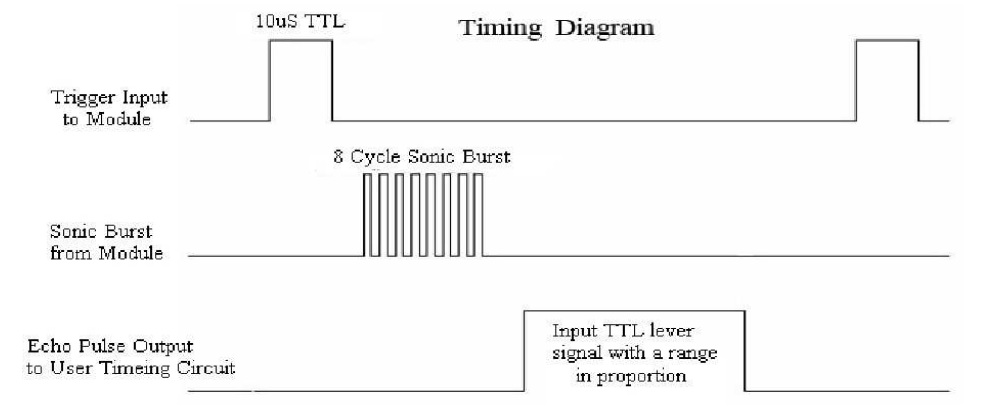
\includegraphics[width=0.5\textwidth]{sonicSensor_timing}
  \caption{Sensor timing diagram \cite{datasheetHCSR04}}
  \label{fig:sonicSensor_timing}
\end{figure}